\documentclass{book}
\usepackage{amsmath}
\usepackage{pgfplots}
\pgfplotsset{compat=newest}

\title {}
\author{}
\date{}


\begin{document}
f: R -> R 
Real valued function

or y = f(x)

Vector-Valued Function: r : R -> Value
r(t) = <f(t), g(t), h(t)>

input is real h


Output is a Vector
Each function components f, g, h ar real valued functions



Generally r(t) = <f(t), g(t), h(t)> = f(t)i + g(t)j + h(t)k>

Example: 
$r(t) = <2+3t, -t, 1+2t>$

Example:
Find the domain of $r(t) = <sqrt(9-t^2), ln(t), e^t>$

Domain of $f(t)=sqrt(9-t^2): 9-t^2 > 0 -> [-3, 3]$

Domain of $ln(t): t > 0$

Domain of $h(t) = e^t: (-infinity, infinity)$


Needs to be in the domain for all three functions
$(0, 3] or  0  < t <= 3$


\textbf{Limits}\\
\\If $r(t) = <f(t), g(t), h(t)>$ then
$lim t->a r(t) = <lim t->a f(t), lim t->a g(t), lim t->a h(t)>$ if each limit exists

Example:
$lim t-> 0+ (tan(t)i + cos(t)j = 1/t k)$
0i + 1j + undefined 
Which means the limit doesn't exist becaues lim t->0+ 1/t = +infinity



Example:
$\lim_{t \to \infty} < e^-t, \frac{2t-1}{3t+2}, tan^-1(t) >$

$= <0, 2/3, pi/2>$

\textbf{Continuity}

Definition: A vector-valued function r(t) is ocntinous at the point given by t=a if 
$\lim_{t \to a} r(t) = r(a)$



Means 3 things are true
1 $\lim_{t \to a} r(t) exists$\\
2 $r(a) \text{exists} (that is, a is in the domain of r(t))$\\
3 limit equals the function value

\textbf{Plane Curve in 2D}\\
Parametric: x = f(t), y=g(t)

Vector function: r(t) = <f(t), g(t)>

\textbf{Space Curve in 3D}\\
Parametric: $x=f(t), y=g(t), z=h(t)$\\
Vector Function: $\vec{r}(t) = <f(t), g(t), h(t)>$

Example: Sketch the space curve given by $r(t) = 4cos(t)i + 4sin(t)j + tk$

$x=4cost, y=4sint, z=t$
z increases as t increases
\begin{align}
    x^2 + y^2 = (4cos(t))^2 + (4sin(t))^2\\
    x^2+y^2 = 16cos^2(t) + 16sin^2(t)\\
    x^2 + y^2 = 16(cos^2(t) + sin^2(t))\\
    x^2 + y^2 = 16
\end{align}

cylinder of radius 4 centered at origin

when t=0 @ (4, 0, 0)

the graph looks like a vector spiraling counter-clockwise around a cylinder

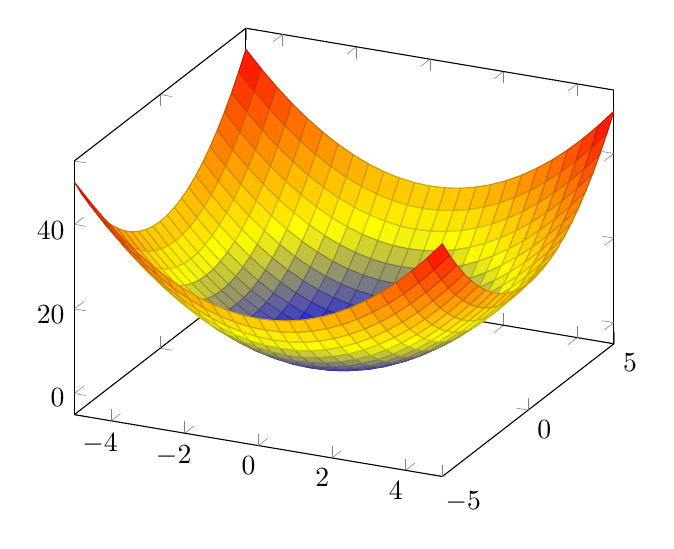
\begin{tikzpicture}
    \begin{axis}
        \addplot3[surf]{x^2 + y^2};
\end{axis}
\end{tikzpicture}



Example:
Find the vector-valued function that represents the intersection of the semi-ellipsoid
\begin{align}
    x^2/12 + y^2/24 + z^2/4 = 1, z>= 0 \\
    \text{parabolic cylinder} y = x^2
\end{align}

\begin{align}
    \text{Parametrize equation for parabolic cylinder:}
    \text{Let x=t}
    \text{Then }y=t^2
    \text{Substitute into equation for semiellipsoid}
    \frac{t^2}{12} + \frac{(t^2)^2}{24} + \frac{z^2}{4} = 1 
    \text{Solve for z}
    $2t^2 + t^4 + 6z^2 = 24 => z^2 = \frac{(24 - 2t^2 - 4t^2)}{6}$
\end{align}


r(t) = <t, t^2, sqrt((24-2t^2-t^4)/4)>
z = sqrt((24-2t^2-t^4)/6)


\textbf{Derivatives}
dr/dt = r'(t) = lim h->0 (r(t+h) - r(t))/h

= lim h->0 < (f(t+h) - f(t))/h, (g(t+h) - g(t))/h, (H(t+h) - H(t))/h >
= <f'(t), g'(t), h'(t) >

r'(t) is tangent to the curve at t

unit tangent vector T(t) = r'(t)/|r'(t)|

\end{document}